\section{Introduction}
\begin{quotation}
	\raggedleft \it
	Black holes are where God divided by zero \\
	-- Anonymous et al.
\end{quotation}
It is well accepted that the centres of many galaxies harbour a super-massive compact dark object \cite{ref_centralobjects}.
The masses of roughly 20 such objects, located in inactive galaxies, have been established to lie in the range between
$10^6 \rightarrow 3\times 10^9M_\odot$ \cite{ref_centralobjectsbiggest}. The radii of these objects are less well determined.
Studies of the variability of the luminosities of active galactic nuclei place upper limits on their radii of a few $10^{-2}$pc
\cite{ref_centralobjects}.

\subsection{The Sgr A Complex}
In the case of the nearest super-massive compact dark object at the centre of the Milky Way, one can, based on the statistics of
proper motion of the stars in the central cluster, conclude that a dark mass of $\sim 2.6 \times 10^6 M_\odot$
must be within 0.015pc from the dynamical centre of the galaxy \cite{ref_ghezmotion}.

The central region of our own galaxy is Sgr A
(Figure \ref{fig_radio}). It consists of three main parts, Sgr A West (Figure \ref{fig_sgrawest}), Sgr A East (Figure \ref{fig_sgraeast})
and a very strong radio source known as Sgr A*, believed by many to be a black hole. The proper motion of Sgr A* has been established
to be smaller than 20km/s \cite{ref_radioproper}. In order to maintain this small velocity for an extended period of time, the mass of
Sgr A* needs to be larger than $10^3M_\odot$. Moreover, Very Large Baseline Array (VLBA) measurements indicate that the radio emission
takes place within a region of a few AU \cite{ref_vlba}.

\begin{figure}[p]
	\begin{center}
	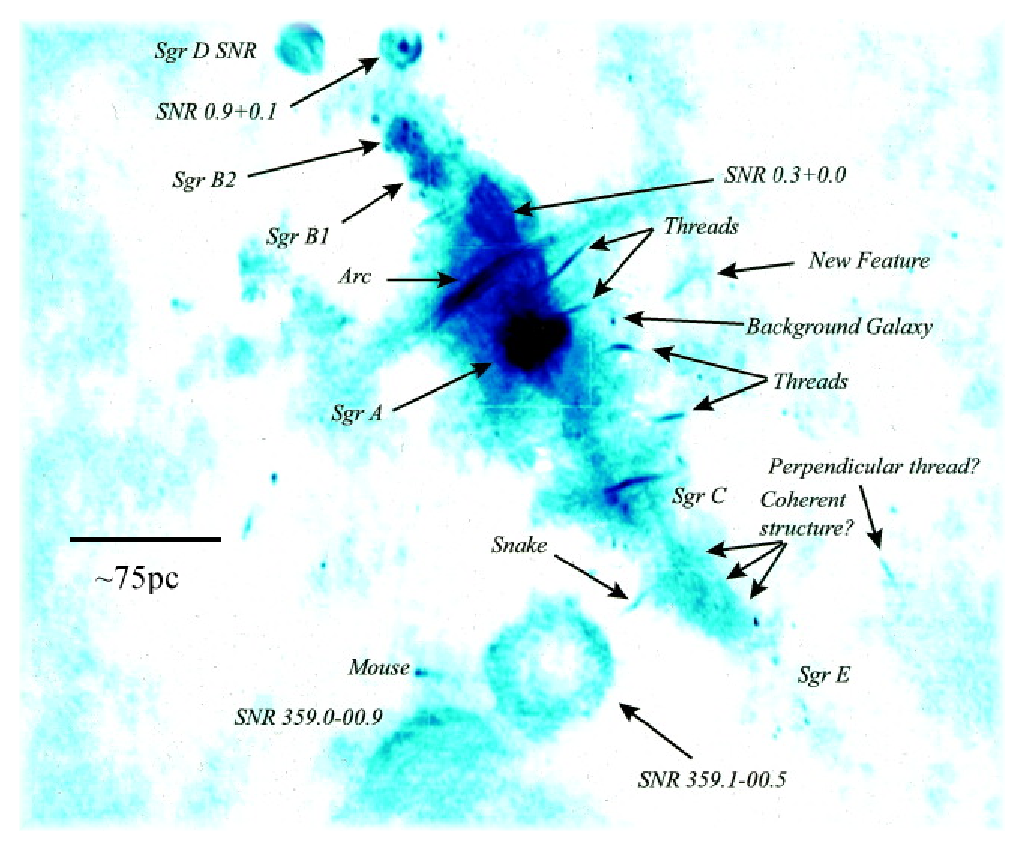
\includegraphics[angle=0,width=0.6\textwidth]{eps/radio.eps}
	\caption{Wide field radio image of the central region of the Milky Way, performed at $\lambda$=90cm \cite{ref_radiopic}.}
	\label{fig_radio}
	\end{center}
\end{figure}
\begin{figure}[p]
	\begin{center}
	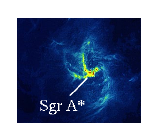
\includegraphics[angle=0,width=0.6\textwidth]{eps/sgrawest.eps}
	\caption{$\lambda$=6cm image of Sgr A. Close to Sgr A* lies a collection of filamentary structures known as Sgr A West.
	The emission from Sgr A West is due to ionised gas that is heated by the numerous young, hot stars in the region.
	(Image courtesy of Prof. K. Y. Lo, University of Illinois).}
	\label{fig_sgrawest}
	\end{center}
\end{figure}
\begin{figure}[p]
	\begin{center}
	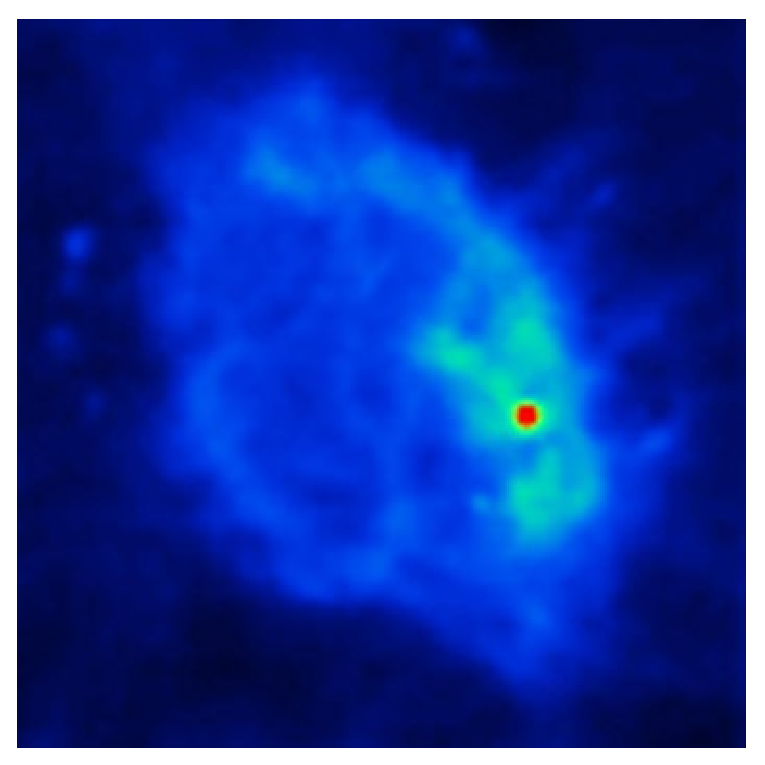
\includegraphics[angle=0,width=0.6\textwidth]{eps/sgraeast.eps}
	\caption{$\lambda$=20cm image of Sgr A. The light blue, shell-like feature (Sgr A East) is thought to be a supernova remnant. The
	red point in the image is the Sgr A* radio source (Image courtesy of R. Plante, University of Illinois).}
	\label{fig_sgraeast}
	\end{center}
\end{figure}
\begin{figure}[p]
	\begin{center}
	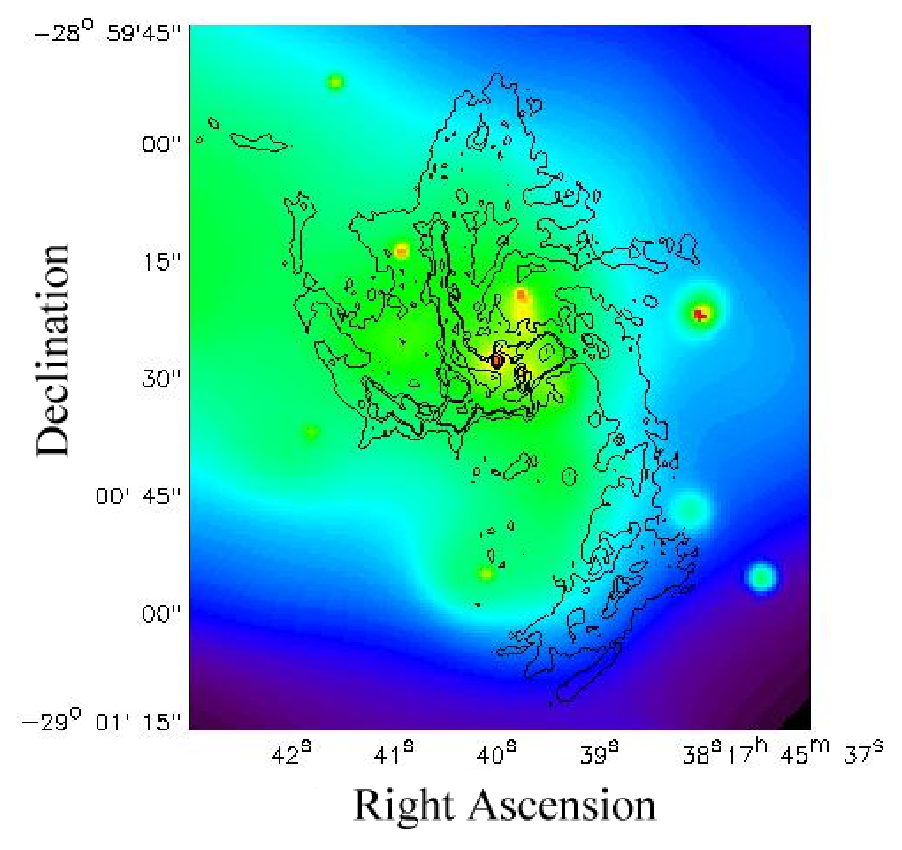
\includegraphics[angle=0,width=0.6\textwidth]{eps/xray.eps}
	\caption{0.5$\rightarrow$7keV image of the central region of the Milky Way. The image has been adaptively smoothed and flat-fielded.
	Overlaid on the image are $\lambda$=6cm contours from Figure \ref{fig_sgrawest}. X-ray emission from the vicinity of Sgr A*
	appears as a red dot at $\rm 17^h45^m40.0^s$, $-29^000'28''$ (J2000.0) \cite{ref_baganoffsubmit}.}
	\label{fig_xray}
	\end{center}
\end{figure}
\begin{figure}[t]
	\begin{center}
	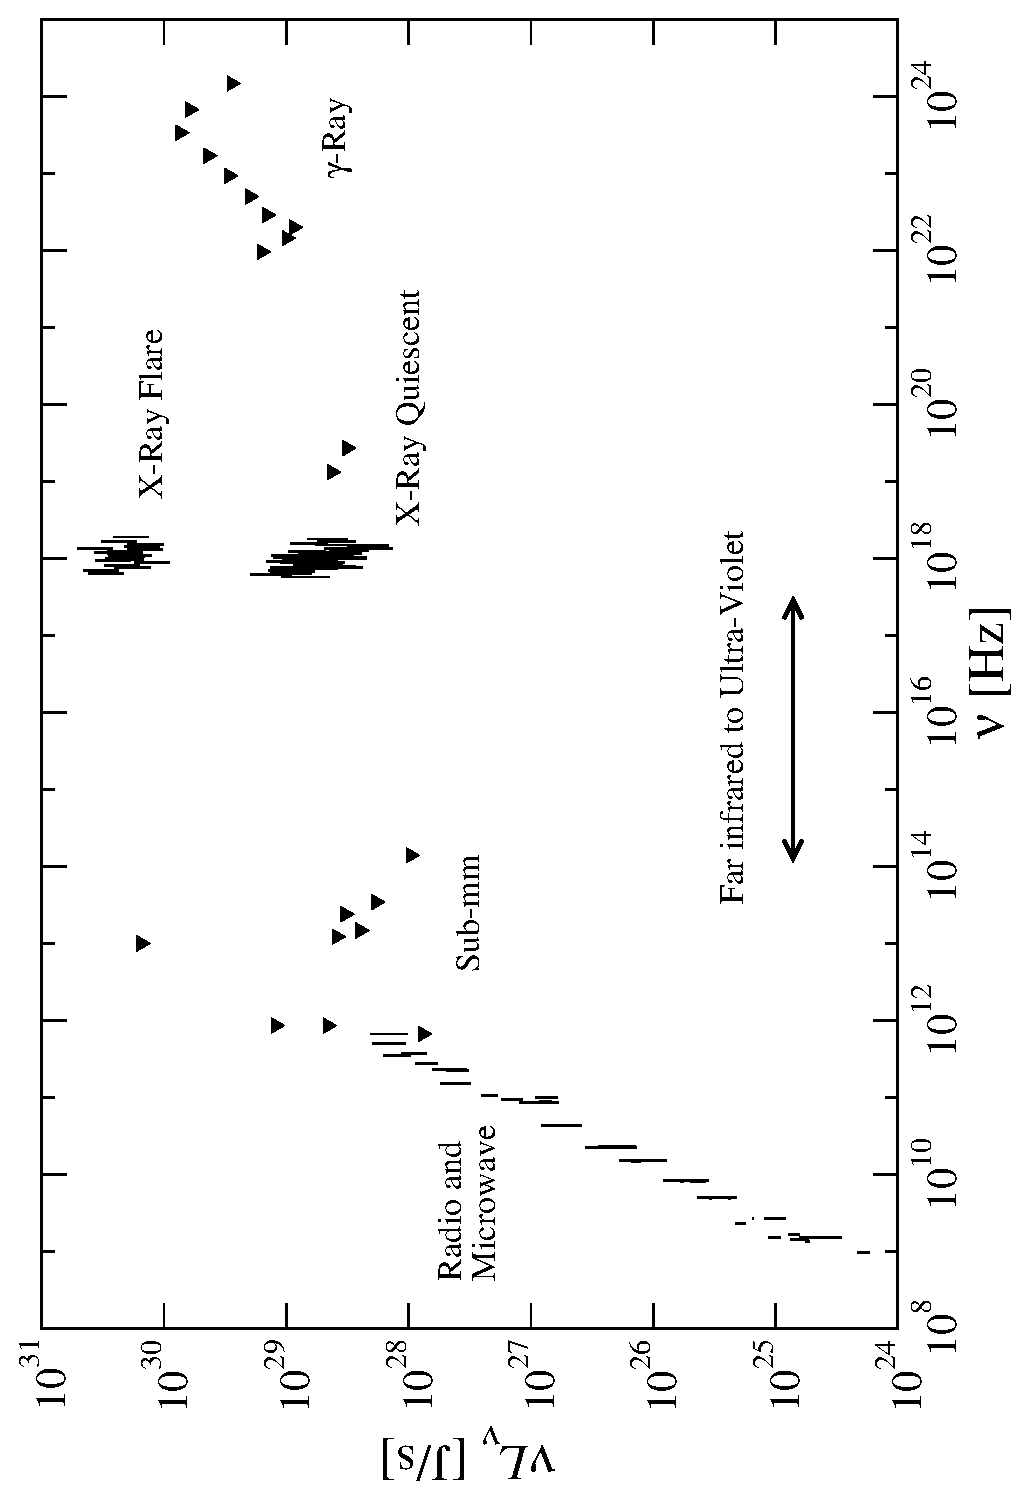
\includegraphics[angle=-90,width=0.9\textwidth]{eps/submm-nuL.eps}
	\caption{Compilation of spectral data in the direction of Sgr A. Triangular data points are upper limits \cite{ref_cokerthesis}.}
	\label{fig_compiledspectrum}
	\end{center}
\end{figure}

Sgr A* has been extensively studied at various wavelengths. The X-ray region (Figure \ref{fig_xray}) is of great importance
as it reveals an interesting `flaring' of the spectrum.
A compilation of spectral data is presented in Figure \ref{fig_compiledspectrum}.
The infra-red (IR), optical and ultraviolet (UV) regions are devoid of detected emission. In the optical and UV regions,
this is solely due to the enormous amount of Galactic foreground extinction.

\subsection{Alternatives to the Black Hole Scenario}
It is natural to speculate that the objects observed in other galaxies are the same as the object at our own galactic centre. The
most commonly accepted idea is that Sgr A* is a black hole. The formation of such super-massive black holes prior to the onset of the
quasar era (z $\approx$ 6) still remains a mystery. Thus until an event horizon is actually observed, it is important to study
alternative scenarios.

Most of the alternative scenarios to the black hole paradigm of Sgr A* usually concentrate either on
predictions of the spectrum, or dynamics of the cluster stars. Some of these ideas and their associated problems are briefly discussed.

One idea that has already been explored is that of a super-massive star consisting of normal matter, with an even heavier accretion disk
\cite{ref_kundt}. This scenario meets problems in explaining the IR spectrum. A compact and dark stellar
cluster has also been proposed as a solution \cite{ref_maoz}. Such a cluster requires evaporation and collision time-scales larger
than the lifetime of our galaxy. This is more likely to be fulfilled using a cluster of sub-stellar objects.
Some alternatives have even touched upon the bizarre, such as the claim of a `white hole' at our galactic centre \cite{ref_whitehole}.
% Said as if a fermion ball isn't bizzare!!

An interesting theory uses neutralinos to explain dark matter evolution and distribution in the galaxy \cite{ref_neutralino}.
The neutralino is postulated as the main component of dark matter. The neutralino is the lightest
SuSy particle, a superposition of the photino, zino and the super-partners of the neutral scalar Higgs particles.
\begin{eqnarray*}
	\chi = N_1\widetilde{\gamma} + N_2\widetilde{Z^0} + N_3\widetilde{H^0_1} + N_4\widetilde{H^0_2}
\end{eqnarray*}
It is stable due to R-parity conservation, and should have a mass $\sim$ 100GeV.
This theory predicts a non-dissipative gravitational singularity or `spike' at the centre of our galaxy, but this has not been observed. The
annihilation processes would result in a distinctive $\gamma$-ray and radio spectrum. As the $\gamma$-ray maps of the galactic centre
are somewhat incomplete and of low resolution, and also due to the shear scale of this theory, much more investigation (far beyond the
scope of the galactic centre) is required in order to test it fully.

In a `from scratch' approach to postulating the form of a super-massive compact dark object, it is vital to look at the object's
composition. It is natural, considering the incredible masses involved, to postulate that the objects are made from the most
fundamental of stable particles, as opposed to some exotic blend. The particle world consists of bosons and fermions.
If we consider a single ingredient particle then the super-massive objects will be either bosonic or fermionic.

A self-gravitating, degenerate, `fermion ball' has already been proposed
\cite{ref_fermion1, ref_fermion2, ref_fermion3, ref_thomasfermiapproach, ref_bilic, ref_classicalapproach}.
As the constituent particles are all fermions, Pauli's Exclusion
Principle dictates that the particles exert a degeneracy pressure upon each other, which counteracts the gravitational force.
In contrast to the proposed fermion ball, a `boson star' has also been presented in \cite{ref_bosonstar}, the Heisenberg
uncertainty principle keeping the system from collapsing into a black hole.
However such boson stars are limited in maximal mass by a $M \sim R^{-1}$ relation as opposed to $M \sim R^{-3}$ for a fermion ball (in a
non-relativistic approach). It is therefore impossible for the boson stars to explain the most massive objects in galactic centres (such
as M87 in the Virgo cluster \cite{ref_centralobjects}) as well as the least massive such as Sgr A*. A fermion ball is capable of
explaining both the most and least massive of the objects through 16keV fermions.

\subsection{Fermion Candidates}
Although this thesis will treat the fermion ball as consisting of an undetected neutral, massive fermion, it is worthwhile to comment
on possible candidates for such a particle. If such a particle does not exist, then the fermion ball scenario is obviously an impossible one.
We will see later that we require a fermion of mass $\sim$ 16keV, and this will be the main factor in discriminating candidates. It is
therefore clear that the neutralino is not a viable candidate as it has a predicted mass in the GeV range.

The most obvious neutral fermion is the neutron. However, it has a mass of 940MeV, which is much too high for our requirements.

Neutrino stars, have been postulated as far back as 1964 \cite{ref_neutrinostar}, in order to explain
quasars. Unfortunately, the mass of active neutrinos are too small to be candidates for the galactic fermion ball. Present upper
limits are $\le$2.2eV for each of the 3 light species \cite{ref_neutrinomass,ref_neutrinomass2}.
Only 3 active neutrinos can exist on account of
limits on the invisible decay width of the $Z^0$ boson \cite{ref_4neutrinos}.
It has also been shown that if the dark matter in the universe were comprised of
neutrinos of mass $\sim$ 16keV, it would over-close the universe by orders of magnitude \cite{ref_nonneutrino}. However,
a possible candidate could be a sterile neutrino, which does not participate in weak interactions but is mixed with at least one
active neutrino. For two-neutrino mixing
\begin{eqnarray}
	 | \nu_\alpha \rangle &=& \cos{\theta} | \nu_1 \rangle + \sin{\theta} | \nu_2 \rangle \nonumber \\
	 | \nu_s \rangle &=& -\sin{\theta} | \nu_1 \rangle + \cos{\theta} | \nu_2 \rangle
	 \label{eqn_sterileneutrino}
\end{eqnarray}
where $| \nu_\alpha \rangle$ and $| \nu_s \rangle$ are active ($\alpha = e,\mu,\tau$) and sterile neutrino flavour eigenstates, respectively.
$| \nu_1 \rangle$ and $| \nu_2 \rangle$ are the mass eigenstates with mass eigenvalues $m_1$ and $m_2$ respectively.
Such mixing renders these species not truly sterile and as a result, they can decay.
We require this decay time to be large and therefore the mixing angle to be small.
Sterile neutrinos have been suggested as a candidate for hot, warm or cold dark matter \cite{ref_sterileneutrino1, ref_sterileneutrino},
with a predicted mass range 1keV$\rightarrow$10MeV due to suspicions of multiple generations.

Alternatively the fermion may be either the gravitino, postulated in super-gravity theories with a mass range of 1keV$\rightarrow$100GeV
\cite{ref_gravitino} or the axino with a predicted mass 1keV$\rightarrow$1GeV, as predicted by the super-symmetric extensions of the
Peccei-Quinn solution to the strong CP problem \cite{ref_axinomass, ref_axino, ref_axinodark}.

\subsection{Where do the Fermions Come From?}
It is also important to understand how such a large gathering of fermions could originate.

If we assume a small primordial lepton asymmetry, sterile neutrinos would have been produced non-resonantly at the beginnings of the
universe. Early constraints on production were derived in \cite{ref_sterileneutrinoconstraint1, ref_sterileneutrinoconstraint2}. Analytic
estimates were later made on relic sterile neutrino abundance \cite{ref_sterileneutrinoanalytic}. Active
neutrinos are still produced today, mainly within the nuclear reactions of stars and from natural neutron decay. These active neutrinos
could resonate into the sterile state, as previously mentioned, and therefore yield an additional source of sterile neutrino. This
again however, depends upon the (as yet unknown) decay time of the sterile neutrino.

Gravitinos are created in the early universe with a cosmologically significant abundance. They could be created either thermally after
reheating \cite{ref_gravitinothermal}, or non-thermally from the vacuum fluctuations, before horizon exit during inflation
\cite{ref_gravitinononthermal}.

The axino is a super-symmetric prediction, it can therefore arise from the moment when low energy super-symmetry is softly
broken. Production can be either thermal or non-thermal. Axinos have a predicted lifetime of the order $>10^{40}$years.

Our three candidates are primordially produced in the early universe, and (assuming long lifetimes) are therefore all
acceptable candidates for at least part of the missing dark matter. This thesis will not focus upon the dark matter
implications of the required fermions. However, remarks will be made about effects that an associated fermion halo may have on our
own galaxy's rotation curve problem.

\subsection{Thesis Objectives}
\begin{quotation}
	\raggedleft \it
	Prediction is very difficult, especially of the future.\\
	-- Niels Bohr
\end{quotation}
We start by introducing a formalism for describing the potential and mass distribution within a fermion ball, using Newtonian mechanics.
This will later be extended to a relativistic approach. After discussing the formation theory, this potential will be used to
predict the motions of stars moving within the fermion ball. Comparison will be made with black hole predictions and experimental
observations. We present the data in the form of high resolution $\chi^2$ phase space plots for the unknown position and velocity parameters
in our line of sight.

A simple non-relativistic accretion `toy model' will be developed for each scenario to derive the observed spectrum from Sgr A.

Finally, we remark upon the ability of the fermion halo theory to explain the dark matter distribution within our galaxy.
